
\subsection{Der Mittelwertsatz der Differentialrechnung}
In diesem Abschnitt werden wir
%den Zwischenwertsatz für stetige Funktionen und 
den ersten Mittelwertsatz der Differentialrechnung kennenlernen. Damit werden wir das Restglied der Taylorreihe abschätzen können.

\begin{LA}{}{MWS}
	Betrachten Sie den Graphen der Funktion $f(x) = x^3-x+3$ im Bereich $x\in[-2, 2]$.
	\begin{center}
		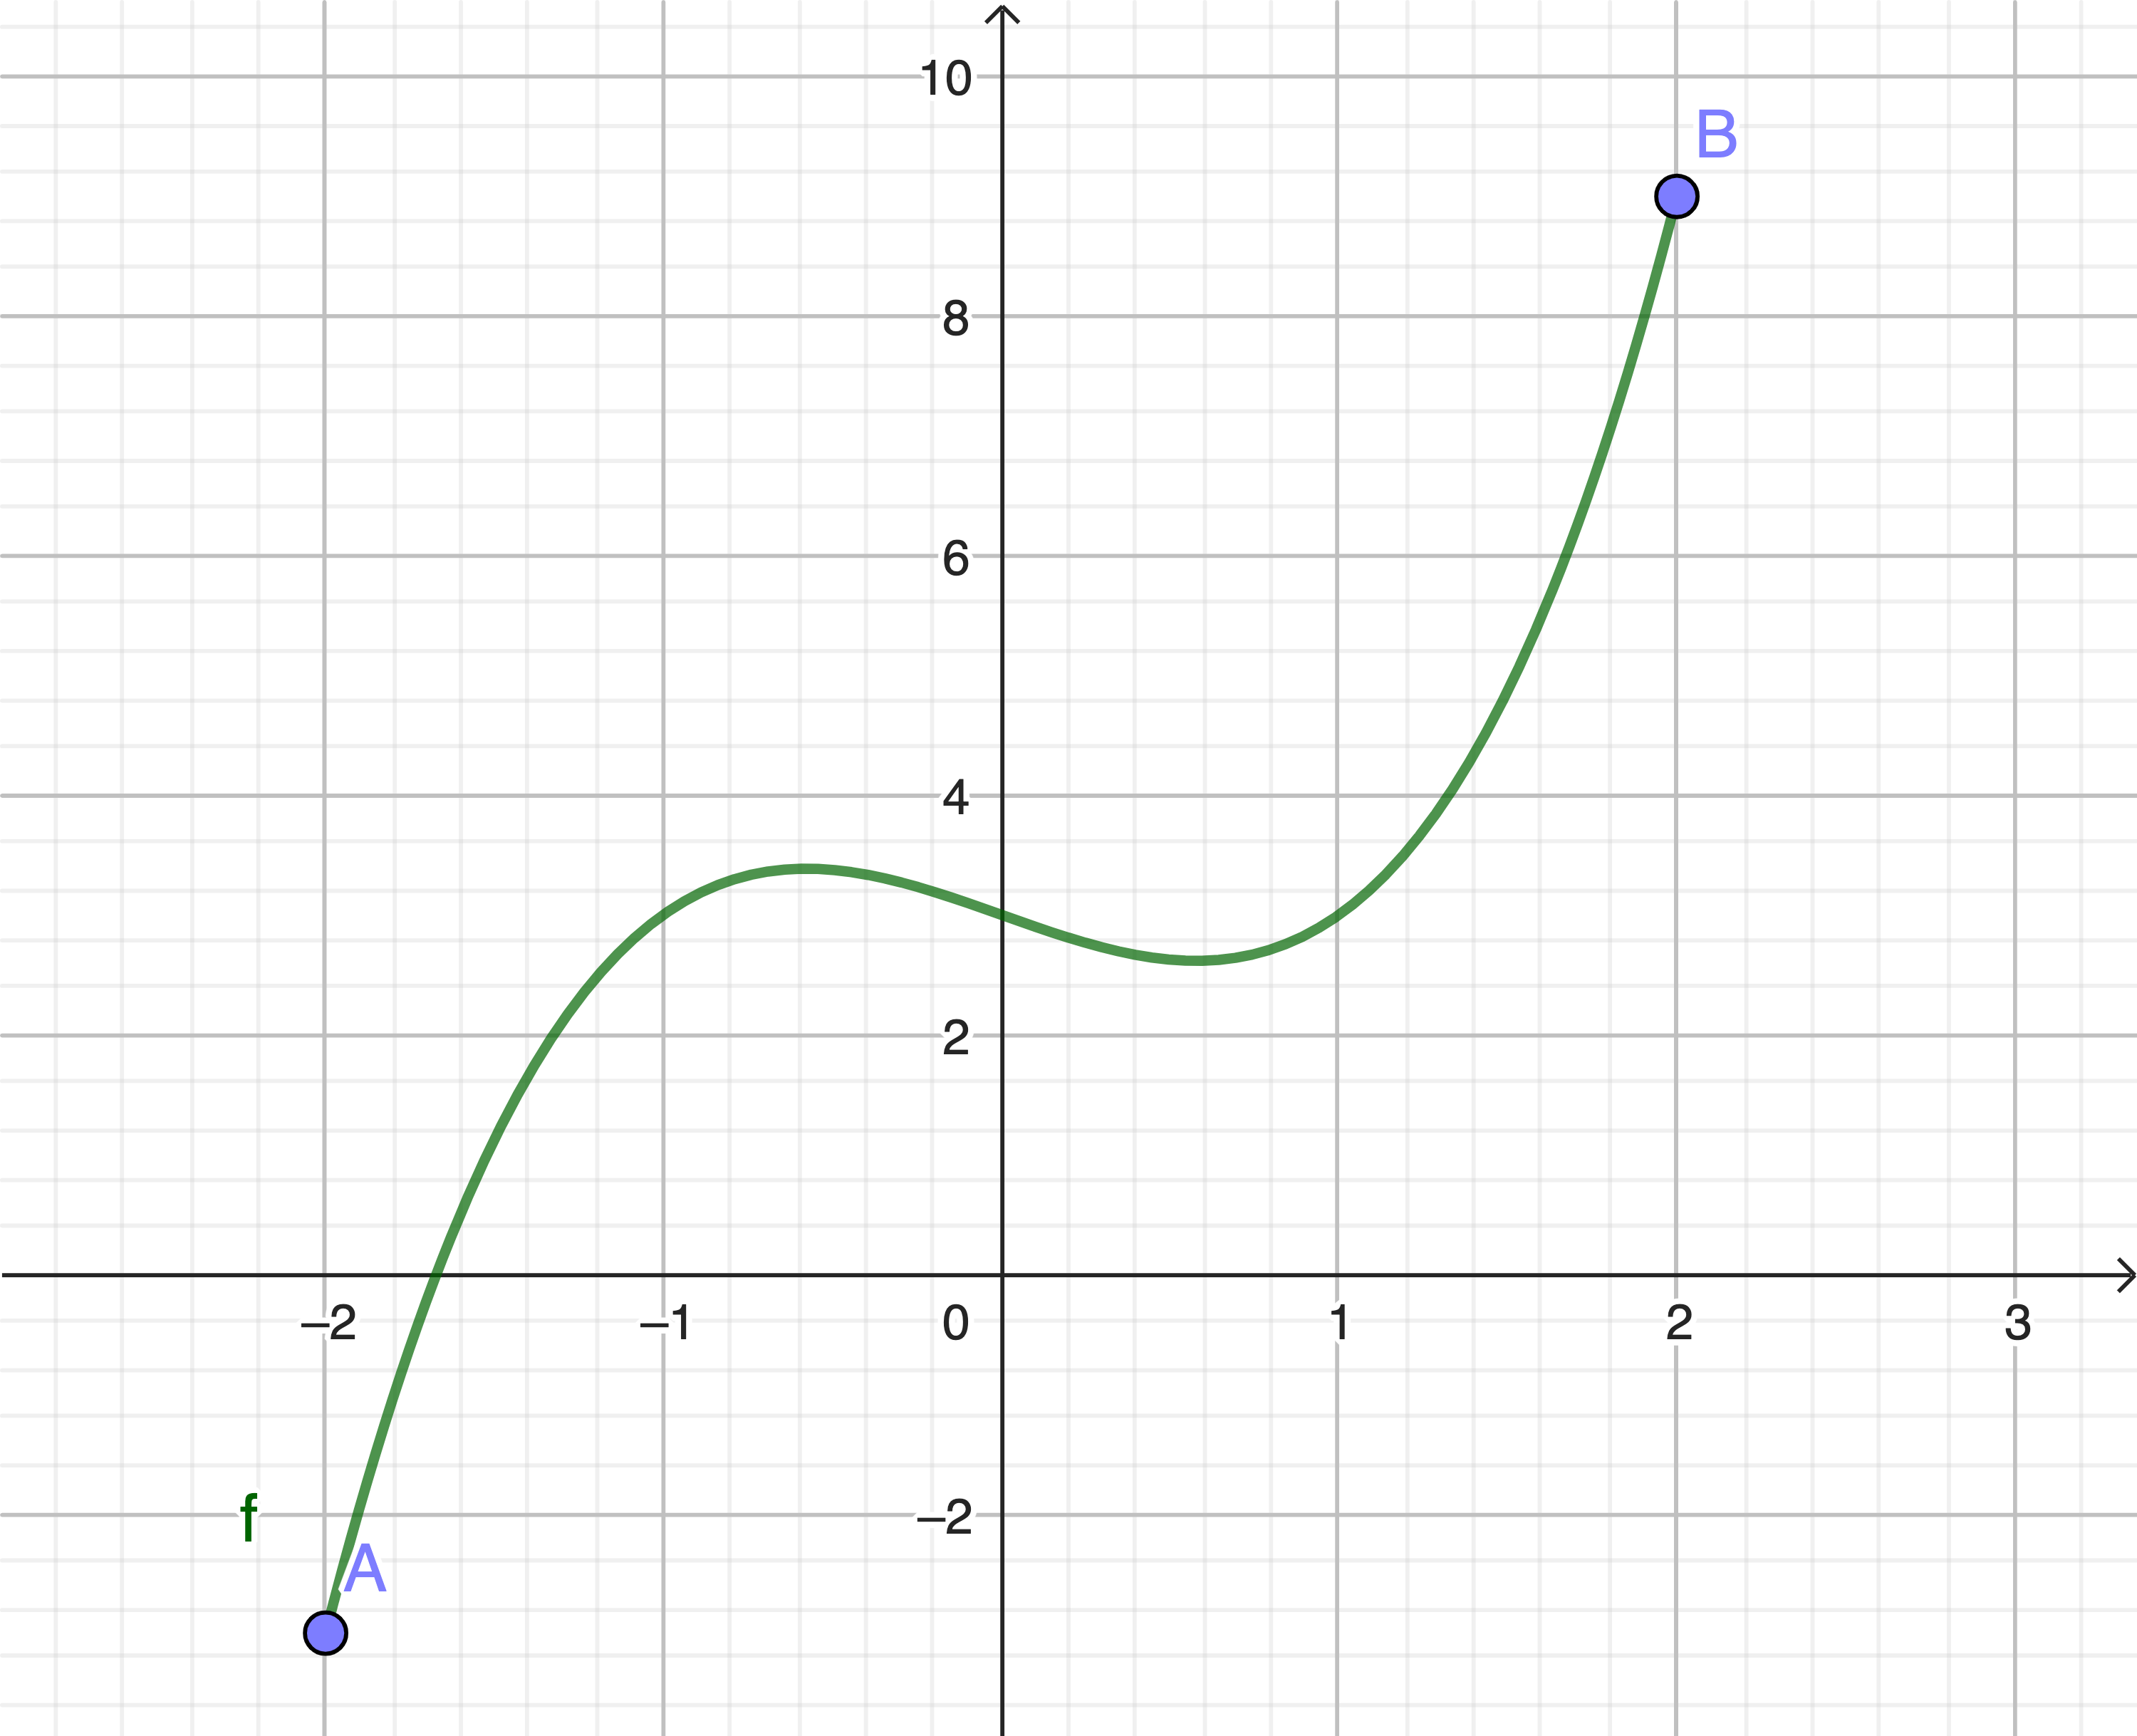
\includegraphics[width = 0.5 \textwidth]{media/LA-MWSV2.png}
	\end{center}

	\begin{enumerate}
		% \item Berechnen Sie den Wert des Quotienten 
		%     $$ \frac{\Delta y}{\Delta x} = \frac{f(2)-f(-2)}{2-(-2)} $$
		%     Welche geometrische Bedeutung hat dieser Zahl im Bezug auf den Graphen von $f$?
		\item Berechnen Sie die Steigung $m$ der Strecke zwischen den beiden Endpunkten $A$ und $B$ des Graphen von $f$.
		\item Schätzen Sie mit dem Graphen, an welchen Stellen der Graph von $f$ die Steigung $m$ aufweist.
		%\item Berechnen Sie den exakten Wert der Stellen, an welchen Stellen der Graph von $f$ die Steigung $m$ aufweist.
		\item Alice behauptet, sie kenne eine differenzierbare Funktion $f: \, [a,b] \rightarrow \R$ mit der Eigenschaft, dass
		      $$f'(x) > \frac{f(b)-f(a)}{b-a}$$
		      für alle $x\in [a,b]$.

		      Argumentieren Sie, wieso das nicht möglich ist.

	\end{enumerate}

\end{LA}

\clearpage

Die Überlegungen aus der Lernaufgabe können allgemein formuliert werden:

\begin{satz}{Erster Mittelwertsatz}{MWS1}
	Sei $f:[a,b]\longrightarrow \mathbb{R}$ eine stetig differenzierbare Funktion. Dann gibt es ein $c\in ]a,b[$ mit
	$$
		\frac{f(b)-f(a)}{b-a} \; = \; f'(c).
	$$
\end{satz}
Wir verzichten an dieser Stelle auf einen exakten Beweis des Satzes. Stattdessen werden wir ein anschauliches Argument liefern:

Die linke Seite der Gleichung im Satz $m = \frac{f(b)-f(a)}{b-a}$ ist die Steigung der Verbindungsstrecke $s$ zwischen den beiden Endpunkten $A=(a, f(a))$ und $B=(b, f(b))$ des Graphen. Diese kann auch interpretiert werden als die mittlere Steigung der Funktion $f$ im Intervall $[a,b]$.

Wenn die lokale Steigung $f'(x_1)$ an einer Stelle $x_1\in ]a,b[$ grösser als die mittlere Steigung $m$ ist, muss dieser Überschuss an einer anderen Stelle $x_2\in ]a,b[$ kompensiert werden.

In anderen Worten: wenn es eine Stelle $x_1$ gibt mit  $f'(x_1)>m$, muss es eine andere Stelle $x_2$ geben mit $f'(x_2) < m$. Da die Ableitungsfunktion $f'$ stetig ist (keine Sprünge aufweist), gibt es zwischen $x_1$ und $x_2$ mindestens eine Stelle $c$ mit $f'(c)=m$.
\begin{center}
	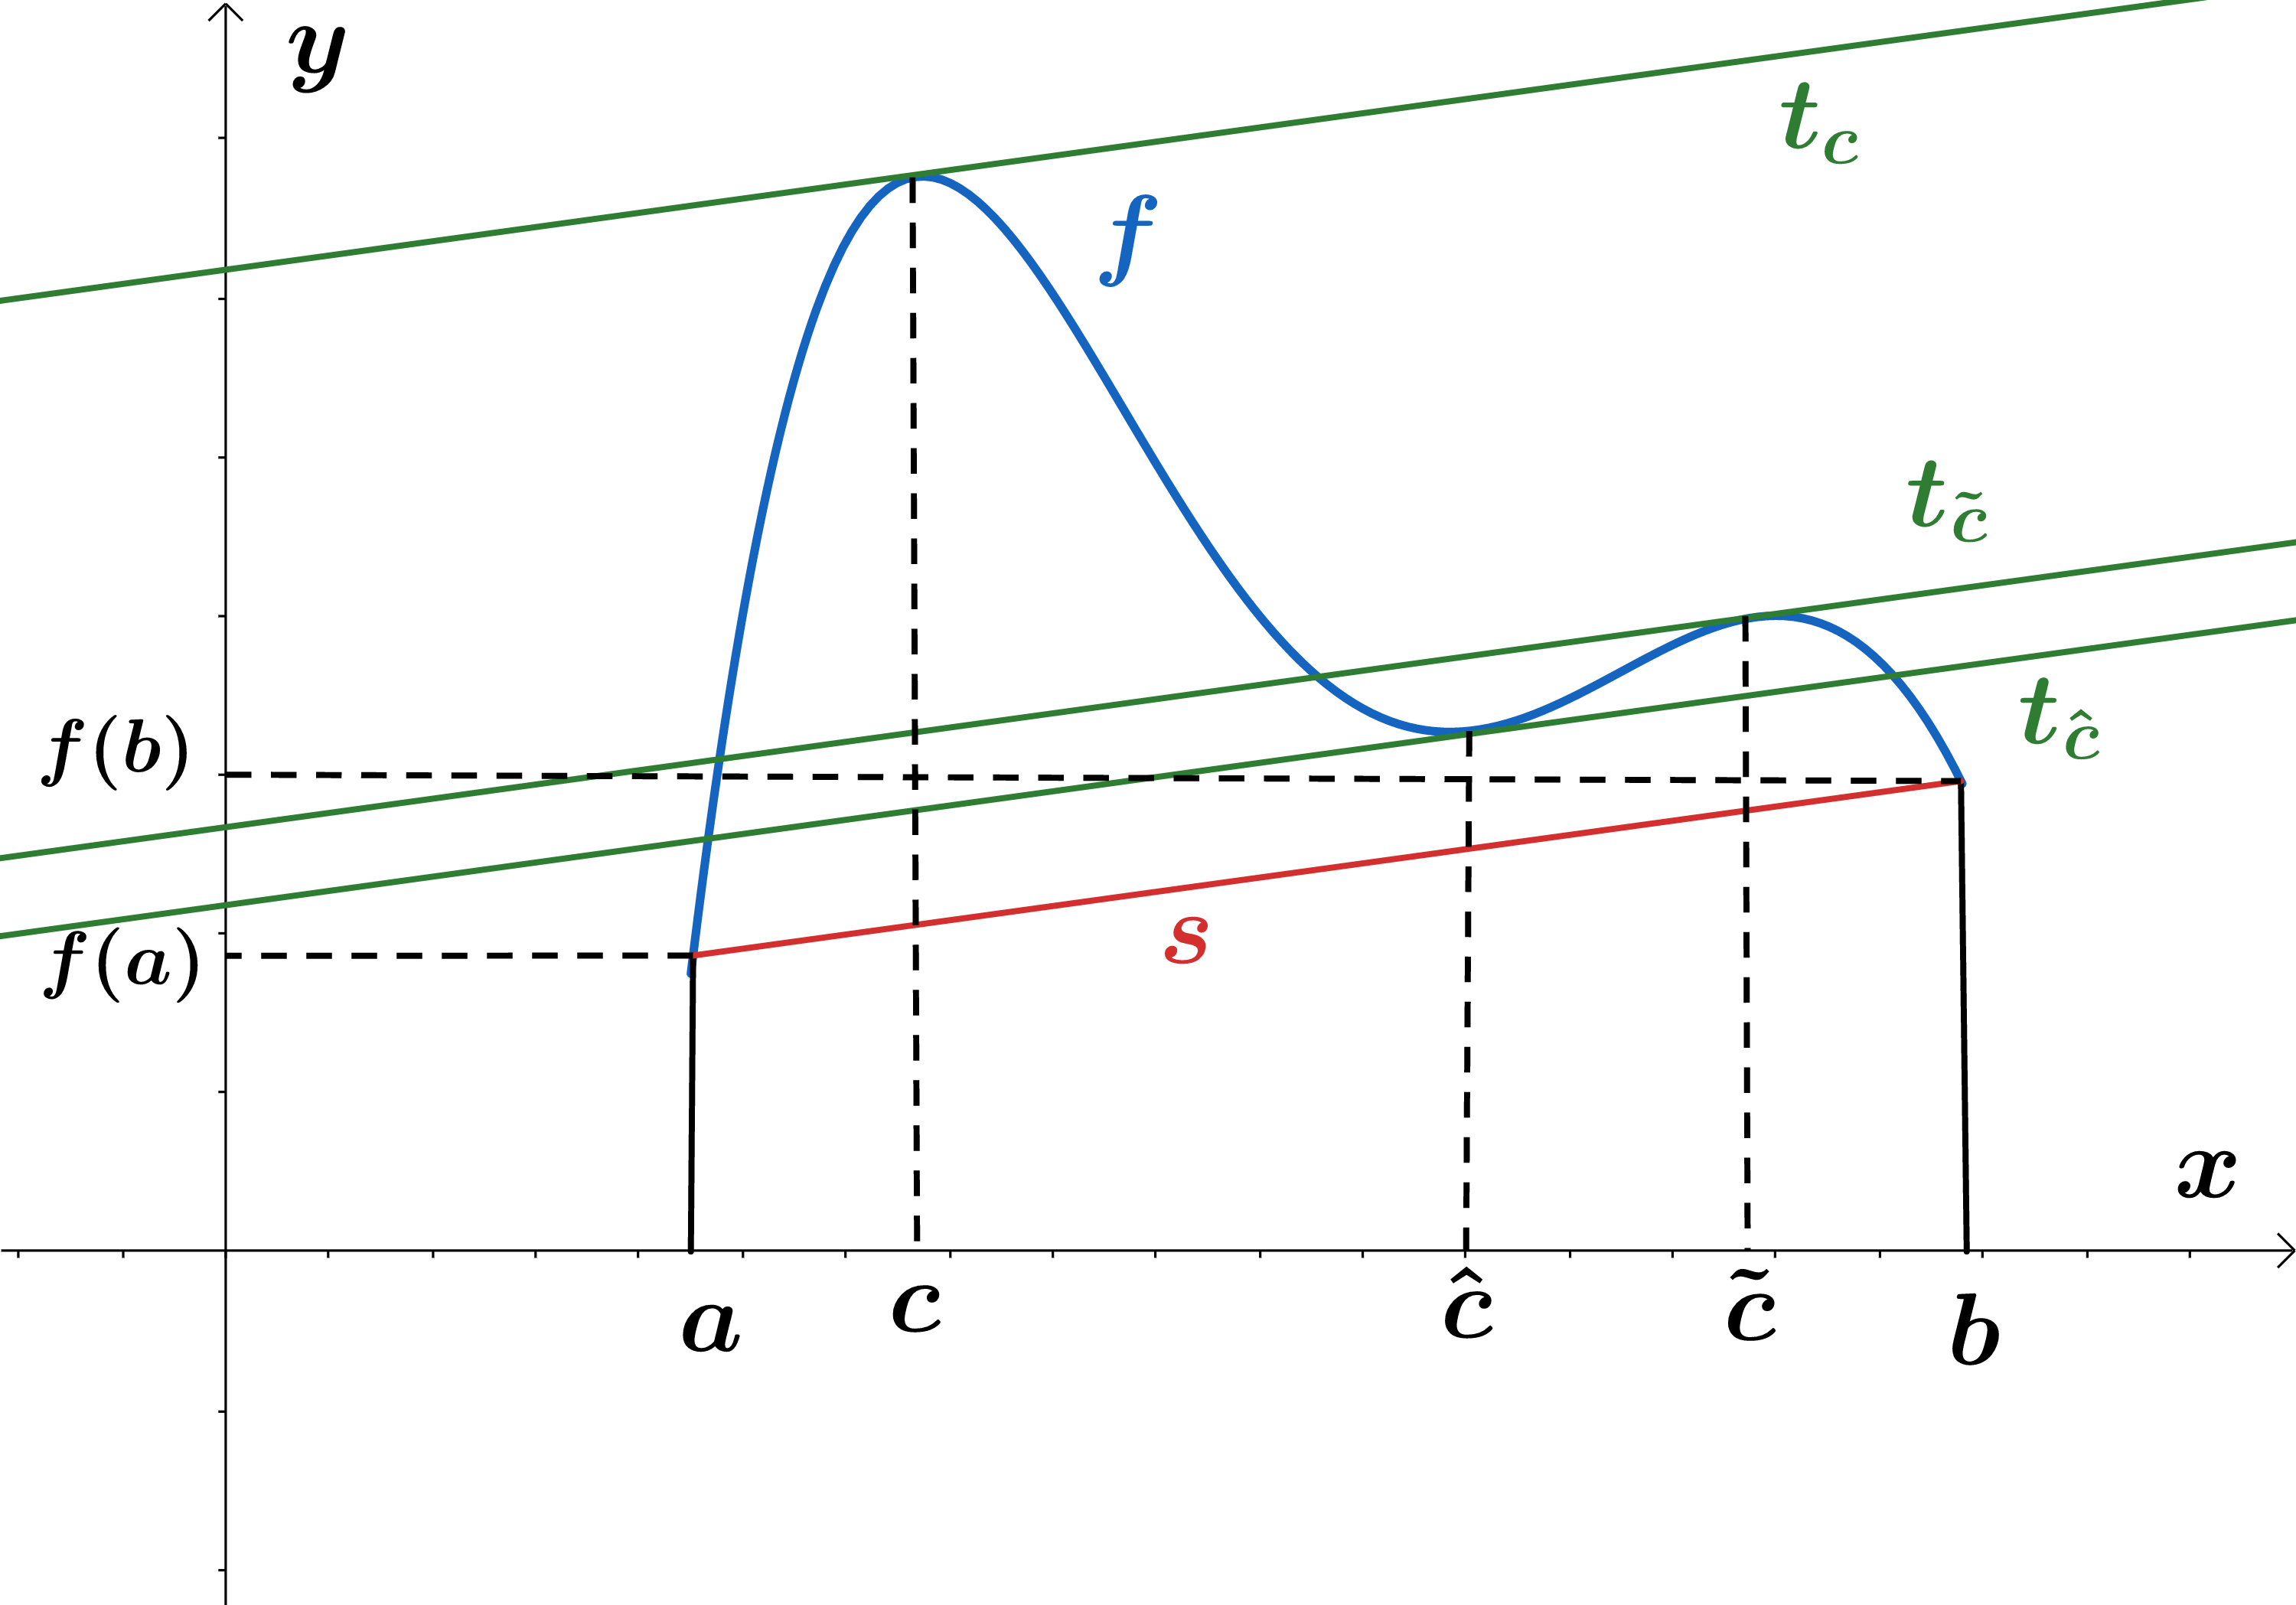
\includegraphics[width = 0.5 \textwidth]{media/mws.png}
\end{center}

Beim ersten Mittelwertsatz handelt es sich um einen sogenannten Existenzsatz. Er besagt zwar, dass eine Stelle $c\in ]a,b[$ mit
$
	\frac{f(b)-f(a)}{b-a} \; = \; f'(c)
$
existiert, gibt aber keine Anleitung, wie man diese Stelle finden kann. Auf den ersten Blick könnte man meinen, dass ein solcher Satz nicht sehr nützlich ist. Tatsächlich kann man aber damit konkrete Aussagen herleiten. Betrachten Sie dazu das folgende Beispiel. Dessen Aussage ist für uns nicht weiter wichtig. Es soll aber exemplarisch zeigen, wie man aus einem Existenzsatz eine konkrete Folgerung ziehen kann:
\clearpage
\begin{bsp}{Eine konkrete Anwendung des Mittelwertsatzes}{}
	Für jede positive Zahl $x > 0$ gilt $e^x > x+1$.
	\vspace{10cm}
	%Diese Ungleichung lässt sich mit dem ersten Mittelwertsatz herleiten.
\end{bsp}



\begin{ueb}{}{}
	Verwenden Sie den ersten Mittelwertsatz, um die folgende Ungleichung zu beweisen: Für alle $x>1$ gilt
	$$1 - \frac{1}{x} < \ln(x) < x-1$$

	Tipp: Die eine Ungleichung findet man, indem man das $c$  im Mittelwertsatz durch $1$ abschätzt, die andere, wenn man $c$ durch $x$ abschätzt.





\end{ueb}
% \clearpage
% \emph{Lösung}
% Das geht analog zum Beispiel. Die eine Ungleichung findet man, indem man das $c$  im Mittelwertsatz durch $1$ abschätzt, die andere, wenn man $c$ durch $x$ abschätzt.





%% Ausführliche Lösung - IGNORE %%
% Betrachte die Funktion \( f(t) = \ln(t) \) im Intervall \([1, x]\). Nach dem ersten Mittelwertsatz der Differentialrechnung gibt es ein \( c \in ]1, x[\) mit
% \[
% 	\frac{\ln(x) - \ln(1)}{x - 1} = \frac{1}{c}
% \]
% Daraus folgt
% \[
% 	\ln(x) = \frac{x}{c} - \frac{1}{c}
% \]
% Wegen \(1 < c < x\) folgt
% \[
% 	\frac{x}{x} - \frac{1}{x} < \ln(x) < \frac{x}{1} - \frac{1}{1}
% \]
% was zu beweisen war.


